\documentclass[a4paper,14pt,oneside,final]{extarticle}
\usepackage[top=2cm, bottom=2cm, left=3cm, right=1cm]{geometry}
\usepackage{scrextend}

\usepackage[T2A,T1]{fontenc}
\usepackage[ukrainian,russian,english]{babel}
\usepackage{tempora}
\usepackage{fontspec}
\setmainfont{tempora}

% Зачем: Отключает использование изменяемых межсловных пробелов.
% Почему: Так не принято делать в текстах на русском языке.
\frenchspacing

\usepackage{indentfirst}
\setlength{\parindent}{1.25cm}
\renewcommand{\baselinestretch}{1.5}

% Header
\usepackage{fancyhdr}
\pagestyle{fancy}
\fancyhead{}
\fancyfoot{}
\fancyhead[R]{\small \selectfont \thepage}
\renewcommand{\headrulewidth}{0pt}

% Captions
\usepackage{chngcntr}
\counterwithin{figure}{section}
\counterwithin{table}{section}
\usepackage[tableposition=top]{caption}
\usepackage{subcaption}
\DeclareCaptionLabelFormat{gostfigure}{Рисунок #2}
\DeclareCaptionLabelFormat{gosttable}{Таблиця #2}
\DeclareCaptionLabelSeparator{gost}{~---~}
\captionsetup{labelsep=gost}
\captionsetup[figure]{labelformat=gostfigure}
\captionsetup[table]{labelformat=gosttable}
\renewcommand{\thesubfigure}{\asbuk{subfigure}}

% Sections
\usepackage[explicit]{titlesec}
\newcommand{\sectionbreak}{\clearpage}

\titleformat{\section}
  {\centering}{\thesection \quad}{0pt}{\MakeUppercase{#1}}
\titleformat{\subsection}[block]
  {\bfseries}{\thesubsection \quad #1}{0cm}{}

\titlespacing{\section} {0cm}{0cm}{21pt}
\titlespacing{\subsection} {\parindent}{21pt}{0cm}
\titlespacing{\subsubsection} {\parindent}{0cm}{0cm}

% Lists
\usepackage{enumitem}
\renewcommand\labelitemi{--}
\setlist[itemize]{noitemsep, topsep=0pt, wide}
\setlist[enumerate]{noitemsep, topsep=0pt, wide, label=\arabic*}
\setlist[description]{labelsep=0pt, noitemsep, topsep=0pt, leftmargin=2\parindent, labelindent=\parindent, labelwidth=\parindent, font=\normalfont}

% Toc
\usepackage{tocloft}
\tocloftpagestyle{fancy}
\renewcommand{\cfttoctitlefont}{}
\setlength{\cftbeforesecskip}{0pt}
\renewcommand{\cftsecfont}{}
\renewcommand{\cftsecpagefont}{}
\renewcommand{\cftsecleader}{\cftdotfill{\cftdotsep}}

\usepackage{float}
\usepackage{pgfplots}
\usepackage{graphicx}
\usepackage{multirow}
\usepackage{amssymb,amsfonts,amsmath,amsthm}
\usepackage{csquotes}

\usepackage{listings}
\lstset{basicstyle=\footnotesize\ttfamily,breaklines=true}
\lstset{language=Matlab}

\usepackage[
	backend=biber,
	sorting=none,
	language=auto,
	autolang=other
]{biblatex}
\DeclareFieldFormat{labelnumberwidth}{#1}


\newcommand{\labnumber}{1} % first lab
\documentclass[a4paper,14pt,oneside,final]{extarticle}
\usepackage[top=2cm, bottom=2cm, left=3cm, right=1cm]{geometry}
\usepackage{scrextend}

\usepackage[T2A,T1]{fontenc}
\usepackage[ukrainian,russian,english]{babel}
\usepackage{tempora}
\usepackage{fontspec}
\setmainfont{tempora}

% Зачем: Отключает использование изменяемых межсловных пробелов.
% Почему: Так не принято делать в текстах на русском языке.
\frenchspacing

\usepackage{indentfirst}
\setlength{\parindent}{1.25cm}
\renewcommand{\baselinestretch}{1.5}

% Header
\usepackage{fancyhdr}
\pagestyle{fancy}
\fancyhead{}
\fancyfoot{}
\fancyhead[R]{\small \selectfont \thepage}
\renewcommand{\headrulewidth}{0pt}

% Captions
\usepackage{chngcntr}
\counterwithin{figure}{section}
\counterwithin{table}{section}
\usepackage[tableposition=top]{caption}
\usepackage{subcaption}
\DeclareCaptionLabelFormat{gostfigure}{Рисунок #2}
\DeclareCaptionLabelFormat{gosttable}{Таблиця #2}
\DeclareCaptionLabelSeparator{gost}{~---~}
\captionsetup{labelsep=gost}
\captionsetup[figure]{labelformat=gostfigure}
\captionsetup[table]{labelformat=gosttable}
\renewcommand{\thesubfigure}{\asbuk{subfigure}}

% Sections
\usepackage[explicit]{titlesec}
\newcommand{\sectionbreak}{\clearpage}

\titleformat{\section}
  {\centering}{\thesection \quad}{0pt}{\MakeUppercase{#1}}
\titleformat{\subsection}[block]
  {\bfseries}{\thesubsection \quad #1}{0cm}{}

\titlespacing{\section} {0cm}{0cm}{21pt}
\titlespacing{\subsection} {\parindent}{21pt}{0cm}
\titlespacing{\subsubsection} {\parindent}{0cm}{0cm}

% Lists
\usepackage{enumitem}
\renewcommand\labelitemi{--}
\setlist[itemize]{noitemsep, topsep=0pt, wide}
\setlist[enumerate]{noitemsep, topsep=0pt, wide, label=\arabic*}
\setlist[description]{labelsep=0pt, noitemsep, topsep=0pt, leftmargin=2\parindent, labelindent=\parindent, labelwidth=\parindent, font=\normalfont}

% Toc
\usepackage{tocloft}
\tocloftpagestyle{fancy}
\renewcommand{\cfttoctitlefont}{}
\setlength{\cftbeforesecskip}{0pt}
\renewcommand{\cftsecfont}{}
\renewcommand{\cftsecpagefont}{}
\renewcommand{\cftsecleader}{\cftdotfill{\cftdotsep}}

\newcommand{\khpistudentgroup}{КН-34г}
\newcommand{\khpistudentname}{Чепурний~А.~С.}

\newcommand{\khpidepartment}{Програмна інженерія та інформаційні технології управління}
\newcommand{\khpititlewhat}{
	Лабораторна робота №\labnumber \\
	з предмету <<Моделювання систем>>
}
\newcommand{\khpititlewho}{
	Виконав: \\
	\hspace*{\parindent} ст. групи \khpistudentgroup \\
	\hspace*{\parindent} \khpistudentname \\
	Перевірила: \\
	\hspace*{\parindent} ст. в. каф. ПІІТУ \\
	\hspace*{\parindent} Єршова~С.~І. \\
	\hspace*{\parindent} ас. каф. ПІІТУ \\
	\hspace*{\parindent} Литвинова~Ю.~С. \\
}



\usepackage{../packages/tikz-uml}

\graphicspath{{figures/}}

\begin{document}
\Ukrainian

\begin{titlepage}

\begin{center}
	МІНІСТЕРСТВО ОСВІТИ І НАУКИ УКРАЇНИ \\
	НАЦІОНАЛЬНИЙ ТЕХНІЧНИЙ УНІВЕРСИТЕТ \\
	«ХАРКІВСЬКИЙ ПОЛІТЕХНІЧНИЙ ІНСТИТУТ» \\[0.5cm]
	Кафедра <<\khpidepartment>> \\
\end{center}

\vspace{6cm}

\begin{center}
	\khpititlewhat
\end{center}

\vspace{3cm}

\begin{addmargin}[10cm]{0cm}
	\khpititlewho
\end{addmargin}

\vspace{\fill}

\begin{center}
	Харків \the\year
\end{center}

\end{titlepage}

\addtocounter{page}{1}

\section*{Знайомство з середовищем Visual Paradigm for UML}
\subsubsection*{Мета роботи}
Отримати практичні навички роботи в середовищі візуального моделювання Visual Paradigm for UML.
\subsubsection*{Хід роботи}
\begin{enumerate}
\item Ознайомитися із методичними рекомендаціями щодо роботи в середовищі Visual Paradigm for UML.
\item Дослідити можливості Visual Paradigm for UML щодо створення різних типів діаграм.
\item Створити за допомогою Visual Paradigm for UML діаграми компонентів, активності, класів та прецедентів. 
Зберегти проект.
\item Оформити звіт про виконання лабораторної роботи.
\end{enumerate}

\subsection{Діаграма прецедентів}
Приклад діаграми прецедентів представлено на рисунку~\ref{fig:uml_usecase}.

\begin{figure}[H]
    \centering
    \tikzumlset{font=\footnotesize} 
    \tikzumlset{fill usecase=white}
    \begin{tikzpicture} 
        \umlactor[x=4, y=2]{Актор} 
        \umlusecase[x=1, y=0, width=3.5cm, name=import]{Імпорт конфігурації з JADE файлу} 
        \umlusecase[x=0, y=3, width=3.5cm, name=export]{Експорт конфігурації до JADE файлу}

        \umlusecase[x=1, y=6, width=3cm, name=correction]{Коригування моделі рішень актору} 
        \umlusecase[x=7, y=1, name=report]{Генерація звіту} 
        \umlusecase[x=7, y=6, width=3cm, name=current]{Перегляд поточної конфігурації} 
        
        \umlusecase[x=11, y=5, name=report_c_period]{Вибір періоду} 
        \umlusecase[x=9, y=3, name=report_c]{Конфігурація звіту} 
        \umlusecase[x=11, y=1, name=report_c_actors]{Вибір акторів}  

        \umlassoc{Актор}{import}
        \umlassoc{Актор}{export}
        \umlassoc{Актор}{correction}
        \umlassoc{Актор}{report}
        \umlassoc{Актор}{current}

        \umlinclude{report}{report_c}
        \umlextend{report_c_period}{report_c}
        \umlextend{report_c_actors}{report_c}
    \end{tikzpicture}

    \caption{Діаграма прецедентів у UML-нотації}
    \label{fig:uml_usecase}
\end{figure}

\subsection{Діаграма компонентів}
Приклад діаграми прецедентів представлено на рисунку~\ref{fig:uml_component}.

\begin{figure}[H]
    \centering
    \tikzumlset{font=\footnotesize} 
    \tikzumlset{fill component=white}
    \begin{tikzpicture} 
        \begin{umlcomponent}[name=jade,x=-5]{JADE}
            \begin{umlcomponent}{Agent}
                \umlbasiccomponent{Prediction}
            \end{umlcomponent}
        \end{umlcomponent}
        \umlbasiccomponent[name=jadec, x=4]{Controller}
        \umlbasiccomponent[name=json, x=8]{JSON Parser}
        
        \begin{umlcomponent}[name=ui,y=4]{Control Panel UI}
            \umlbasiccomponent[name=conrolconf]{Net Configuration}
            \umlbasiccomponent[name=controlintrusion, x=4]{Agent Intrusion}
            \umlbasiccomponent[name=reportcreate, x=8]{Agent Report}
            \umldelegateconnector{reportcreate}{json}
        \end{umlcomponent}

        \umldelegateconnector{ui}{jadec}
        \umlHVHassemblyconnector[interface=IMessage]{jadec}{jade}
    \end{tikzpicture}
    \caption{Діаграма компонентів у UML-нотації}
    \label{fig:uml_component}
\end{figure}

\subsection{Діаграма активності}
Приклад діаграми прецедентів представлено на рисунку~\ref{fig:uml_activity}.

\begin{figure}[H]
  \centering
    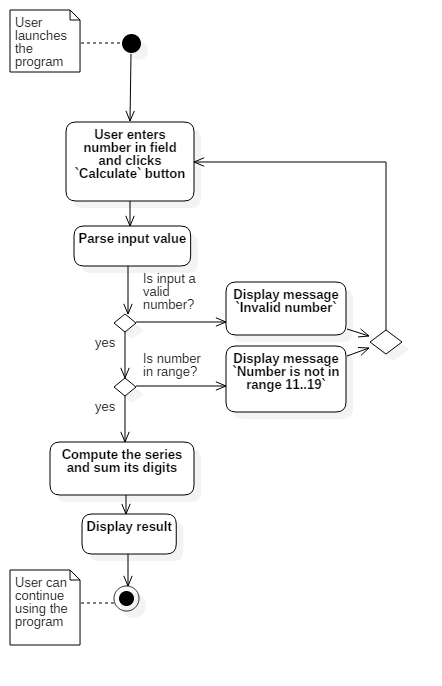
\includegraphics[width=0.6\textwidth]{uml_activity}
  \caption{Діаграма активності у UML-нотації}
  \label{fig:uml_activity}
\end{figure}

\subsection{Діаграма класів}
Приклад діаграми прецедентів представлено на рисунку~\ref{fig:uml_class}.

\begin{figure}[H]
  \centering
    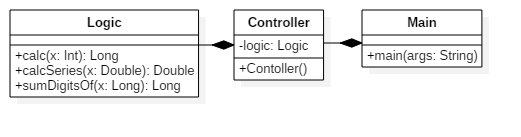
\includegraphics[width=0.8\textwidth]{uml_class}
  \caption{Діаграма класів у UML-нотації}
  \label{fig:uml_class}
\end{figure}

\end{document}
